\documentclass[12pt,a4paper]{article}
\usepackage[a4paper,top=1in,bottom=1in,left=1.25in,right=1.25in]{geometry}
\usepackage{amsmath,latexsym,amssymb,stmaryrd}
\usepackage{amsfonts,amsthm}
\usepackage[utf8]{inputenc}
\usepackage[OT1]{fontenc}
\usepackage[french]{babel} % important pour la typographie et les césures
\usepackage{verbatim,alltt,bm}
\usepackage{xcolor}
\usepackage{tikz}
\usetikzlibrary{arrows,shapes}
\usepackage{hyperref}
\usepackage{fancyhdr}
\usepackage[myheadings]{fullpage}
\setlength{\topmargin}{-1cm}
\setlength{\textheight}{25cm}
\usepackage[linewidth=1pt]{mdframed}
\usepackage[section]{placeins}
\usepackage{graphicx}
\usepackage{subfigure}
\usepackage[titletoc]{appendix}
\usepackage{framed}
\usepackage{minted}
\usepackage{listings}
\newcommand{\tabincell}[2]{\begin{tabular}{@{}#1@{}}#2\end{tabular}}
\usepackage[figuresright]{rotating}
\usepackage{hyperref}
\hypersetup{
    bookmarks=true,         % show bookmarks bar?
    unicode=true,          % non-Latin characters in Acrobat’s bookmarks
    pdftoolbar=true,        % show Acrobat’s toolbar?
    pdfmenubar=true,        % show Acrobat’s menu?
    pdffitwindow=true,     % window fit to page when opened
    pdfstartview={FitH},    % fits the width of the page to the window
    pdftitle={My title},    % title
    pdfauthor={Xicun HAN},     % author
    pdfsubject={Subject},   % subject of the document
    pdfcreator={Xicun HAN},   % creator of the document
    pdfproducer={Producer}, % producer of the document
    pdfkeywords={keyword1, key2, key3}, % list of keywords
    pdfnewwindow=true,      % links in new PDF window
    colorlinks=true,       % false: boxed links; true: colored links
    linkcolor=red,          % color of internal links (change box color with linkbordercolor)
    citecolor=green,        % color of links to bibliography
    filecolor=magenta,      % color of file links
    urlcolor=cyan           % color of external links
}
\definecolor{very-light-gray}{gray}{0.97}

\title{Docker Technical Review}
\author{\\\\\\\\\\\\\\\\\\HAN Xicun\\\\
%Director : Christophe. Rosenberger\\\\
%Informatique M2 , Science\\\\
%University of CAEN \\\\
\texttt{xicun.han@gmail.com}\\\\}
\date{13 Mars 2017}


\begin{document}
	\pagestyle{empty}
	\maketitle
	\thispagestyle{empty}
	\clearpage
	%\pagebreak

	\tableofcontents
	\newpage
	\renewcommand\listoflistingscaption{List of source codes}
	\listoflistings

	\thispagestyle{empty}
	\newpage
	\pagestyle{fancy}
	\lhead{}
	\chead{}
	%\rhead{}
	%\begin{abstract} \setcounter{page}{1}
	%	Ã  remplir
	%\end{abstract}
	\pagebreak
	\FloatBarrier

%\begin{abstract}

%\end{abstract}
\newpage

\section{Basics}

In this section, the following how-to will be discussed: \\

\begin{itemize}
	\item[*] Install Docker for several platforms
	\item[*] Run a software image in a container
	\item[*] browse for an image on Docker Hub
	\item[*] create your own image and run it in a container
	\item[*] create a Docker Hub account and an image repository
	\item[*] Create an Image of your own
	\item[*] Push the image to Docker Hub\\
\end{itemize}

\subsection{Installation}

\subsubsection*{Step 1 Requirements}

\begin{enumerate}
	\item Exam supported Operating systems
	\item Examine Requirement
\end{enumerate}

\subsubsection*{Step 2 Installation}

\begin{itemize}
  \item[*] {\color{red}{Mac OS X}}: \url{https://docs.docker.com/docker-for-mac/install/}
  \item[*] {\color{red}{Windows}} : \url{https://docs.docker.com/docker-for-windows/install/}
  \item[*] {\color{red}{Linux}} : \url{https://docs.docker.com/engine/getstarted/linux_install_help/}
\end{itemize}

\subsubsection*{Step 3: Verify the installation}


\begin{listing}[ht]
 \begin{minted}[frame=lines,
%framesep=2m,
%baselinestretch=1.2,
bgcolor=very-light-gray,
fontsize=\scriptsize,
linenos]{bash}
docker version
docker ps -a

docker run hello-world
\end{minted}
\label{code:1
}
\caption{Verification Installation Docker}
 \end{listing}
\FloatBarrier


\newpage
\subsection{Images and Container}

\begin{figure}[h]
  \begin{center}
    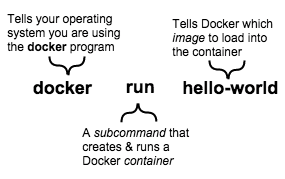
\includegraphics[scale=0.4]{cmd1.png}
    \caption{Command Structure}
    \label{fig:1}
  \end{center}
\end{figure}
\FloatBarrier

\begin{itemize}
  \item[*] An {\color{red}{Image}} is a filesystem and parameters to use at runtime, It doesn't have state and NEVER changes.
  \item[*] A {\color{red}{container}} is a running instance of an image.
\end{itemize}

\begin{listing}[ht]
 \begin{minted}[frame=lines,
%framesep=2m,
%baselinestretch=1.2,
bgcolor=very-light-gray,
fontsize=\scriptsize,
linenos]{bash}

docker run hello-world
Unable to find image 'hello-world:latest' locally
latest: Pulling from library/hello-world78445dd45222: Pull complete
Digest: sha256:c5515758d4c5e1e838e9cd307f6c6a0d620b5e07e6f927b07d05f6d12a1ac8d7
Status: Downloaded newer image for hello-world:latest

Hello from Docker!
This message shows that your installation appears to be working correctly.

To generate this message, Docker took the following steps:
 1. The Docker client contacted the Docker daemon.
 2. The Docker daemon pulled the "hello-world" image from the Docker Hub.
 3. The Docker daemon created a new container from that image which runs the
    executable that produces the output you are currently reading.
 4. The Docker daemon streamed that output to the Docker client, which sent it
    to your terminal.
\end{minted}
\label{code:2}
\caption{Hello World Docker}
 \end{listing}
\FloatBarrier

\newpage


\subsection{Find and Run Whalesay Image}

\subsubsection{Locate Shared Image}
\begin{enumerate}
  \item go to \href{https://hub.docker.com}{Docker Hub}
  \item search for {\color{green}{\textit{docker/whalesay}}}
  \item read about the details on this image. \href{https://hub.docker.com/r/docker/whalesay/}{\underline{details}}
\end{enumerate}

\subsubsection{Run whalesay image}

\begin{enumerate}
  \item open \textit{terminal}
  \item run the commands: {\color{violet}{\textit{docker run docker/whalesay cowsay boo}}}

  \begin{listing}[ht]
   \begin{minted}[frame=lines,
  %framesep=2m,
  %baselinestretch=1.2,
  bgcolor=very-light-gray,
  fontsize=\scriptsize,
  linenos]{bash}
  MBP-de-XICUN $ docker run docker/whalesay cowsay boo$
  Unable to find image 'docker/whalesay:latest' locally
  latest: Pulling from docker/whalesay
  e190868d63f8: Pull complete
  909cd34c6fd7: Pull complete
  0b9bfabab7c1: Pull complete
  a3ed95caeb02: Pull complete
  00bf65475aba: Pull complete
  c57b6bcc83e3: Pull complete
  8978f6879e2f: Pull complete
  8eed3712d2cf: Pull complete
  Digest: sha256:178598e51a26abbc958b8a2e48825c90bc22e641de3d31e18aaf55f3258ba93b
  Status: Downloaded newer image for docker/whalesay:latest
   _____
  < boo >
   -----
      \
       \
        \
                      ##        .
                ## ## ##       ==
             ## ## ## ##      ===
         /""""""""""""""""___/ ===
    ~~~ {~~ ~~~~ ~~~ ~~~~ ~~ ~ /  ===- ~~~
         \______ o          __/
          \    \        __/
            \____\______/


  \end{minted}
  \label{code:3}
  \caption{Result of Running whalesay image}
   \end{listing}
  \FloatBarrier

  \item To look at the images : \textit{{\color{violet}{docker images}}}

  \begin{listing}[ht]
   \begin{minted}[frame=lines,
  %framesep=2m,
  %baselinestretch=1.2,
  bgcolor=very-light-gray,
  fontsize=\scriptsize,
  linenos]{bash}
  MBP-de-XICUN:002_Docker_Learning xicunhan:$ docker images $
  REPOSITORY          TAG                 IMAGE ID            CREATED             SIZE
  hello-world         latest              48b5124b2768        8 weeks ago         1.84 kB
  centos              latest              67591570dd29        2 months ago        192 MB
  ubuntu              16.04               4ca3a192ff2a        3 months ago        128 MB
  docker/whalesay     latest              6b362a9f73eb        21 months ago       247 MB
  \end{minted}
  \label{code:4}
  \caption{Capture Running \textit{Docker images}}
   \end{listing}
  \FloatBarrier

  \item Play with the \emph{whalesay} with a word.

  \begin{listing}[ht]
   \begin{minted}[frame=lines,
  %framesep=2m,
  %baselinestretch=1.2,
  bgcolor=very-light-gray,
   fontsize=\scriptsize,%tiny
  linenos]{bash}
  MBP-de-XICUN:002_Docker_Learning xicunhan\$ docker run docker/whalesay cowsay hello My Friends
   __________________
  < hello My Friends >
   ------------------
      \
       \
        \
                      ##        .
                ## ## ##       ==
             ## ## ## ##      ===
         /""""""""""""""""___/ ===
    ~~~ {~~ ~~~~ ~~~ ~~~~ ~~ ~ /  ===- ~~~
         \______ o          __/
          \    \        __/
            \____\______/

  \end{minted}
  \label{code:5}
  \caption{Play with WhaleSay}
   \end{listing}
  \FloatBarrier

\end{enumerate}


\subsection{Build Your Own Image}

\subsubsection{Write a DockerFile}

\emph{{\color{orange}{Dockerfile}}} is a \textit{recipe} which describes the:
\begin{itemize}
  \item[-] files
  \item[-] environment
  \item[-] commands that make up an image.
\end{itemize}

Make a new Dockerfile, then input the following texts: \\

\begin{listing}[ht]
 \begin{minted}[frame=lines,
%framesep=2m,
%baselinestretch=1.2,
bgcolor=very-light-gray,
 fontsize=\scriptsize,%tiny
linenos]{bash}
FROM docker/whalesay:latest
RUN apt-get -y update && apt-get install -y fortunes
CMD /usr/games/fortune -a | cowsay
\end{minted}
\label{code:6}
\caption{Docker File text}
 \end{listing}
\FloatBarrier

\subsubsection{Build an image from the Dockerfile}

In this part we are going to use the \textit{{\color{violet}{docker build}}} command. \\

The param \textit{-t} gives the image a tag, and the \emph{.} pointed the current working folder.\\

\begin{listing}[ht]
 \begin{minted}[frame=lines,
%framesep=2m,
%baselinestretch=1.2,
bgcolor=very-light-gray,
 fontsize=\scriptsize,%tiny
linenos]{bash}
MBP-de-XICUN:mydouckerbuild xicunhan\$ docker build -t docker-whale .
Sending build context to Docker daemon 2.048 kB
Step 1/3 : FROM docker/whalesay:latest
 ---> 6b362a9f73eb
Step 2/3 : RUN apt-get -y update && apt-get install -y fortunes
 ---> Running in c16171df9bca
Ign http://archive.ubuntu.com trusty InRelease
Get:1 http://archive.ubuntu.com trusty-updates InRelease [65.9 kB]
Get:2 http://archive.ubuntu.com trusty-security InRelease [65.9 kB]
....

Step 3/3 : CMD /usr/games/fortune -a | cowsay
 ---> Running in 85e777d419f8
 ---> bcffe7293416
Removing intermediate container 85e777d419f8
Successfully built bcffe7293416

\end{minted}
\label{code:7}
\caption{Build An Image From The Dockerfile}
 \end{listing}
\FloatBarrier

\subsubsection{Learn About The Build Process}

\begin{enumerate}
  \item Checking everything it needs to build.\\
  \begin{minted}[frame=lines,
  %framesep=2m,
  %baselinestretch=1.2,
  bgcolor=very-light-gray,
  fontsize=\scriptsize,%tiny
  ]{bash}
Sending build context to Docker daemon 2.048 kB
  \end{minted}
\FloatBarrier
  \item Docker check the existence of image \emph{docker/whalesay}, and the end of each step, an \emph{ID} will be generated.\\
  \begin{minted}[frame=lines,
  %framesep=2m,
  %baselinestretch=1.2,
  bgcolor=very-light-gray,
   fontsize=\scriptsize,%tiny
  %linenos
  ]{bash}
Step 1/3 : FROM docker/whalesay:latest
  ---> 6b362a9f73eb
  \end{minted}
  \FloatBarrier
  \item Then docker start up a {\color{brown}{\textit{temporary container}}} and \emph{RUN} the commands \\
  \begin{minted}[frame=lines,
  %framesep=2m,
  %baselinestretch=1.2,
  bgcolor=very-light-gray,
   fontsize=\scriptsize,%tiny
  %linenos
  ]{bash}
  Step 2/3 : RUN apt-get -y update && apt-get install -y fortunes
   ---> Running in c16171df9bca
  Ign http://archive.ubuntu.com trusty InRelease
  Get:1 http://archive.ubuntu.com trusty-updates InRelease [65.9 kB]
  ....
  Processing triggers for libc-bin (2.19-0ubuntu6.6) ...
 ---> aa68367539ea
Removing intermediate container c16171df9bca
  \end{minted}
  \FloatBarrier
  When the RUN command finished a new layer is created and the intermediate temporary container is removed.
  \item A new intermediate container is created and docker adds a layer for the \emph{CMD line} and finally removes this intermediate container.\\
  \begin{minted}[frame=lines,
  %framesep=2m,
  %baselinestretch=1.2,
  bgcolor=very-light-gray,
   fontsize=\scriptsize,%tiny
  %linenos
  ]{bash}
  Step 3/3 : CMD /usr/games/fortune -a | cowsay
   ---> Running in 85e777d419f8
   ---> bcffe7293416
  Removing intermediate container 85e777d419f8
  Successfully built bcffe7293416
  \end{minted}
  \FloatBarrier

\end{enumerate}

\subsubsection{Run the new docker-whale}

We will take a look at all the images by command: \textit{{\color{violet}{docker images}}}, then run the new image by typing: \textit{{\color{violet}{docker run docker-whale}}}: \\

\begin{minted}[frame=lines,
%framesep=2m,
%baselinestretch=1.2,
bgcolor=very-light-gray,
fontsize=\scriptsize,%tiny
%linenos
]{bash}
MBP-de-XICUN:002_Docker_Learning xicunhan\$ docker images
REPOSITORY          TAG                 IMAGE ID            CREATED             SIZE
docker-whale        latest              bcffe7293416        8 hours ago         275 MB
docker/whalesay     latest              6b362a9f73eb        21 months ago       247 MB
MBP-de-XICUN:002_Docker_Learning xicunhan\$ docker run docker-whale
 _________________________________________
/ We are not a loved organization, but we \
| are a respected one.                    |
|                                         |
\ -- John Fisher                          /
 -----------------------------------------
    \
     \
      \
                    ##        .
              ## ## ##       ==
           ## ## ## ##      ===
       /""""""""""""""""___/ ===
  ~~~ {~~ ~~~~ ~~~ ~~~~ ~~ ~ /  ===- ~~~
       \______ o          __/
        \    \        __/
          \____\______/
MBP-de-XICUN:002_Docker_Learning xicunhan\$ docker run docker-whale
 _______________________________________
/ In Newark the laundromats are open 24 \
\ hours a day!                          /
 ---------------------------------------
    \
     \
      \
                    ##        .
              ## ## ##       ==
           ## ## ## ##      ===
       /""""""""""""""""___/ ===
  ~~~ {~~ ~~~~ ~~~ ~~~~ ~~ ~ /  ===- ~~~
       \______ o          __/
        \    \        __/
          \____\______/

\end{minted}
\FloatBarrier



\subsubsection{Pull or Push the Images}

In order to push or pull the images, we should first sign in \href{https://hub.docker.com}{\underline{Docker Hub}}, then create the repository corresponded.\\

\begin{figure}[h]
\begin{center}
  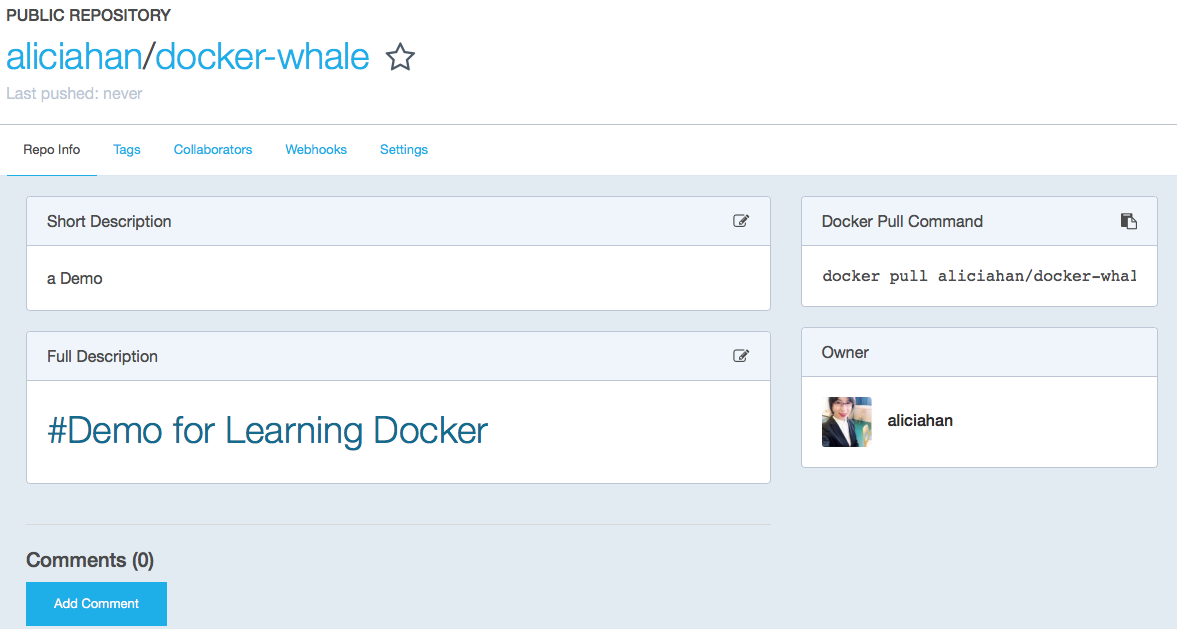
\includegraphics[scale=0.3]{dockerHub.png}
  \caption{Repository Docker Hub}
  \label{fig:2}
\end{center}
\end{figure}
 \FloatBarrier

\textbf{{\color{brown}{To Push an Image:}}}

\begin{enumerate}
  \item Use \textit{{\color{violet}{docker login}}} to Login. \\
  \begin{minted}[frame=lines,
  %framesep=2m,
  %baselinestretch=1.2,
  bgcolor=very-light-gray,
  fontsize=\scriptsize,%tiny
  %linenos
  ]{bash}
  MBP-de-XICUN:002_Docker_Learning xicunhan\$ docker login
  Login with your Docker ID to push and pull images from Docker Hub. If you
  don't have a Docker ID, head over to https://hub.docker.com to create one.
  Username: aliciahan
  Password:
  Login Succeeded
  \end{minted}
  \FloatBarrier

  \item Find the ID and add \textit{{\color{brown}{namespace}}} to the image using \textit{{\color{violet}{docker tag}}} command.\\

  \begin{figure}[h]
  \begin{center}
    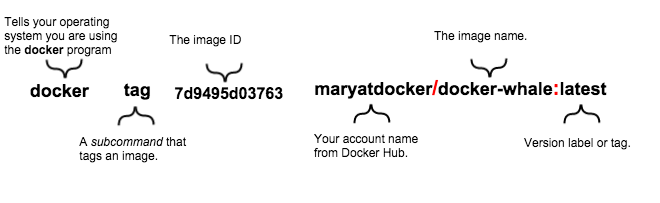
\includegraphics[scale=0.5]{tagger.png}
  \end{center}
  \end{figure}
   \FloatBarrier

  \begin{minted}[frame=lines,
  %framesep=2m,
  %baselinestretch=1.2,
  bgcolor=very-light-gray,
  fontsize=\scriptsize,%tiny
  %linenos
  ]{bash}

  MBP-de-XICUN xicunhan\$ docker images
  REPOSITORY          TAG                 IMAGE ID            CREATED             SIZE
  docker-whale        latest              bcffe7293416        10 hours ago        275 MB

  MBP-de-XICUN xicunhan\$ docker tag bcffe7293416 aliciahan/docker-whale:latest
  MBP-de-XICUN xicunhan\$ docker images
  REPOSITORY               TAG                 IMAGE ID            CREATED             SIZE
  aliciahan/docker-whale   latest              bcffe7293416        10 hours ago        275 MB
  docker-whale             latest              bcffe7293416        10 hours ago        275 MB

  \end{minted}
  \FloatBarrier

  \item Using the \textit{{\color{violet}{docker push aliciahan/docker-whale}}} to Push.
\end{enumerate}

\textbf{{\color{brown}{To Pull an Image:}}}\\

\begin{enumerate}
  \item firstly, remove the images already existe by \textit{{\color{violet}{docker rmi -f $<ID>$}}} or \textit{{\color{violet}{docker image rm -f $<ID>$}}}. \\

  \begin{minted}[frame=lines,
  %framesep=2m,
  %baselinestretch=1.2,
  bgcolor=very-light-gray,
  fontsize=\scriptsize,%tiny
  %linenos
  ]{bash}
  MBP-de-XICUN:xicunhan\$ docker image rm -f bcffe7293416
  Untagged: aliciahan/docker-whale:latest
  Untagged: aliciahan/docker-whale@sha256:1fe4c62848f029b8df04da746031ce1ad586f370769739f011a0035bed036e2f
  Untagged: docker-whale:latest
  Deleted: sha256:bcffe72934167a3147674c250ba59e8de88d8fb947730937ed828489de132677
  Deleted: sha256:aa68367539ea507f7d26d8e0dab3b8a05dd0911a964ccbdc3ec759cfe53a001f
  \end{minted}
  \FloatBarrier

  \item Using \textit{{\color{violet}{Docker run [nameSpace]/[nameRepository]}}} to load the image from the Internet.\\


\end{enumerate}



\section{Define and Deploy Apps}



%\bibliographystyle{IEEEtran}
%\bibliography{biblio}

\end{document}
